\documentclass[english, 11 pt, class=article, crop=false]{standalone}
\usepackage[T1]{fontenc}
%\renewcommand*\familydefault{\sfdefault} % For dyslexia-friendly text
\usepackage{lmodern} % load a font with all the characters
\usepackage{geometry}
\geometry{verbose,paperwidth=16.1 cm, paperheight=24 cm, inner=2.3cm, outer=1.8 cm, bmargin=2cm, tmargin=1.8cm}
\setlength{\parindent}{0bp}
\usepackage{import}
\usepackage[subpreambles=false]{standalone}
\usepackage{amsmath}
\usepackage{amssymb}
\usepackage{esint}
\usepackage{babel}
\usepackage{tabu}
\makeatother
\makeatletter

\usepackage{titlesec}
\usepackage{ragged2e}
\RaggedRight
\raggedbottom
\frenchspacing

% Norwegian names of figures, chapters, parts and content
\addto\captionsenglish{\renewcommand{\figurename}{Figur}}
\makeatletter
\addto\captionsenglish{\renewcommand{\chaptername}{Kapittel}}
\addto\captionsenglish{\renewcommand{\partname}{Del}}


\usepackage{graphicx}
\usepackage{float}
\usepackage{subfig}
\usepackage{placeins}
\usepackage{cancel}
\usepackage{framed}
\usepackage{wrapfig}
\usepackage[subfigure]{tocloft}
\usepackage[font=footnotesize,labelfont=sl]{caption} % Figure caption
\usepackage{bm}
\usepackage[dvipsnames, table]{xcolor}
\definecolor{shadecolor}{rgb}{0.105469, 0.613281, 1}
\colorlet{shadecolor}{Emerald!15} 
\usepackage{icomma}
\makeatother
\usepackage[many]{tcolorbox}
\usepackage{multicol}
\usepackage{stackengine}

\usepackage{esvect} %For vectors with capital letters

% For tabular
\usepackage{array}
\usepackage{multirow}
\usepackage{longtable} %breakable table

% Ligningsreferanser
\usepackage{mathtools}
\mathtoolsset{showonlyrefs}

% index
\usepackage{imakeidx}
\makeindex[title=Indeks]

%Footnote:
\usepackage[bottom, hang, flushmargin]{footmisc}
\usepackage{perpage} 
\MakePerPage{footnote}
\addtolength{\footnotesep}{2mm}
\renewcommand{\thefootnote}{\arabic{footnote}}
\renewcommand\footnoterule{\rule{\linewidth}{0.4pt}}
\renewcommand{\thempfootnote}{\arabic{mpfootnote}}

%colors
\definecolor{c1}{cmyk}{0,0.5,1,0}
\definecolor{c2}{cmyk}{1,0.25,1,0}
\definecolor{n3}{cmyk}{1,0.,1,0}
\definecolor{neg}{cmyk}{1,0.,0.,0}

% Lister med bokstavar
\usepackage[inline]{enumitem}

\newcounter{rg}
\numberwithin{rg}{chapter}
\newcommand{\reg}[2][]{\begin{tcolorbox}[boxrule=0.3 mm,arc=0mm,colback=blue!3] {\refstepcounter{rg}\phantomsection \large \textbf{\therg \;#1} \vspace{5 pt}}\newline #2  \end{tcolorbox}\vspace{-5pt}}

\newcommand\alg[1]{\begin{align} #1 \end{align}}

\newcommand\eks[2][]{\begin{tcolorbox}[boxrule=0.3 mm,arc=0mm,enhanced jigsaw,breakable,colback=green!3] {\large \textbf{Eksempel #1} \vspace{5 pt}\\} #2 \end{tcolorbox}\vspace{-5pt} }

\newcommand{\st}[1]{\begin{tcolorbox}[boxrule=0.0 mm,arc=0mm,enhanced jigsaw,breakable,colback=yellow!12]{ #1} \end{tcolorbox}}

\newcommand{\spr}[1]{\begin{tcolorbox}[boxrule=0.3 mm,arc=0mm,enhanced jigsaw,breakable,colback=yellow!7] {\large \textbf{Språkboksen} \vspace{5 pt}\\} #1 \end{tcolorbox}\vspace{-5pt} }

\newcommand{\sym}[1]{\colorbox{blue!15}{#1}}

\newcommand{\info}[2]{\begin{tcolorbox}[boxrule=0.3 mm,arc=0mm,enhanced jigsaw,breakable,colback=cyan!6] {\large \textbf{#1} \vspace{5 pt}\\} #2 \end{tcolorbox}\vspace{-5pt} }

\newcommand\algv[1]{\vspace{-11 pt}\begin{align*} #1 \end{align*}}

\newcommand{\regv}{\vspace{5pt}}
\newcommand{\mer}{\textsl{Merk}: }
\newcommand{\mers}[1]{{\footnotesize \mer #1}}
\newcommand\vsk{\vspace{11pt}}
\newcommand\vs{\vspace{-11pt}}
\newcommand\vsb{\vspace{-16pt}}
\newcommand\sv{\vsk \textbf{Svar} \vspace{4 pt}\\}
\newcommand\br{\\[5 pt]}
\newcommand{\figp}[1]{../fig/#1}
\newcommand\algvv[1]{\vs\vs\begin{align*} #1 \end{align*}}
\newcommand{\y}[1]{$ {#1} $}
\newcommand{\os}{\\[5 pt]}
\newcommand{\prbxl}[2]{
\parbox[l][][l]{#1\linewidth}{#2
	}}
\newcommand{\prbxr}[2]{\parbox[r][][l]{#1\linewidth}{
		\setlength{\abovedisplayskip}{5pt}
		\setlength{\belowdisplayskip}{5pt}	
		\setlength{\abovedisplayshortskip}{0pt}
		\setlength{\belowdisplayshortskip}{0pt} 
		\begin{shaded}
			\footnotesize	#2 \end{shaded}}}

\renewcommand{\cfttoctitlefont}{\Large\bfseries}
\setlength{\cftaftertoctitleskip}{0 pt}
\setlength{\cftbeforetoctitleskip}{0 pt}

\newcommand{\bs}{\\[3pt]}
\newcommand{\vn}{\\[6pt]}
\newcommand{\fig}[1]{\begin{figure}
		\centering
		\includegraphics[]{\figp{#1}}
\end{figure}}

\newcommand{\figc}[2]{\begin{figure}
		\centering
		\includegraphics[]{\figp{#1}}
		\caption{#2}
\end{figure}}

\newcommand{\sectionbreak}{\clearpage} % New page on each section

\newcommand{\nn}[1]{
\begin{equation}
	#1
\end{equation}
}

% Equation comments
\newcommand{\cm}[1]{\llap{\color{blue} #1}}

\newcommand\fork[2]{\begin{tcolorbox}[boxrule=0.3 mm,arc=0mm,enhanced jigsaw,breakable,colback=yellow!7] {\large \textbf{#1 (forklaring)} \vspace{5 pt}\\} #2 \end{tcolorbox}\vspace{-5pt} }
 
%colors
\newcommand{\colr}[1]{{\color{red} #1}}
\newcommand{\colb}[1]{{\color{blue} #1}}
\newcommand{\colo}[1]{{\color{orange} #1}}
\newcommand{\colc}[1]{{\color{cyan} #1}}
\definecolor{projectgreen}{cmyk}{100,0,100,0}
\newcommand{\colg}[1]{{\color{projectgreen} #1}}

% Methods
\newcommand{\metode}[2]{
	\textsl{#1} \\[-8pt]
	\rule{#2}{0.75pt}
}

%Opg
\newcommand{\abc}[1]{
	\begin{enumerate}[label=\alph*),leftmargin=18pt]
		#1
	\end{enumerate}
}
\newcommand{\abcs}[2]{
	\begin{enumerate}[label=\alph*),start=#1,leftmargin=18pt]
		#2
	\end{enumerate}
}
\newcommand{\abcn}[1]{
	\begin{enumerate}[label=\arabic*),leftmargin=18pt]
		#1
	\end{enumerate}
}
\newcommand{\abch}[1]{
	\hspace{-2pt}	\begin{enumerate*}[label=\alph*), itemjoin=\hspace{1cm}]
		#1
	\end{enumerate*}
}
\newcommand{\abchs}[2]{
	\hspace{-2pt}	\begin{enumerate*}[label=\alph*), itemjoin=\hspace{1cm}, start=#1]
		#2
	\end{enumerate*}
}

% Oppgaver
\newcommand{\opgt}{\phantomsection \addcontentsline{toc}{section}{Oppgaver} \section*{Oppgaver for kapittel \thechapter}\vs \setcounter{section}{1}}
\newcounter{opg}
\numberwithin{opg}{section}
\newcommand{\op}[1]{\vspace{15pt} \refstepcounter{opg}\large \textbf{\color{blue}\theopg} \vspace{2 pt} \label{#1} \\}
\newcommand{\ekspop}[1]{\vsk\textbf{Gruble \thechapter.#1}\vspace{2 pt} \\}
\newcommand{\nes}{\stepcounter{section}
	\setcounter{opg}{0}}
\newcommand{\opr}[1]{\vspace{3pt}\textbf{\ref{#1}}}
\newcommand{\oeks}[1]{\begin{tcolorbox}[boxrule=0.3 mm,arc=0mm,colback=white]
		\textit{Eksempel: } #1	  
\end{tcolorbox}}
\newcommand\opgeks[2][]{\begin{tcolorbox}[boxrule=0.1 mm,arc=0mm,enhanced jigsaw,breakable,colback=white] {\footnotesize \textbf{Eksempel #1} \\} \footnotesize #2 \end{tcolorbox}\vspace{-5pt} }
\newcommand{\rknut}{
Rekn ut.
}

%License
\newcommand{\lic}{\textit{Matematikken sine byggesteinar by Sindre Sogge Heggen is licensed under CC BY-NC-SA 4.0. To view a copy of this license, visit\\ 
		\net{http://creativecommons.org/licenses/by-nc-sa/4.0/}{http://creativecommons.org/licenses/by-nc-sa/4.0/}}}

%referances
\newcommand{\net}[2]{{\color{blue}\href{#1}{#2}}}
\newcommand{\hrs}[2]{\hyperref[#1]{\color{blue}\textsl{#2 \ref*{#1}}}}
\newcommand{\rref}[1]{\hrs{#1}{regel}}
\newcommand{\refkap}[1]{\hrs{#1}{kapittel}}
\newcommand{\refsec}[1]{\hrs{#1}{seksjon}}

\newcommand{\mb}{\net{https://sindrsh.github.io/FirstPrinciplesOfMath/}{MB}}


%line to seperate examples
\newcommand{\linje}{\rule{\linewidth}{1pt} }

\usepackage{datetime2}
%%\usepackage{sansmathfonts} for dyslexia-friendly math
\usepackage[]{hyperref}


\newcommand{\note}{Merk}
\newcommand{\notesm}[1]{{\footnotesize \textsl{\note:} #1}}
\newcommand{\ekstitle}{Eksempel }
\newcommand{\sprtitle}{Språkboksen}
\newcommand{\expl}{forklaring}

\newcommand{\vedlegg}[1]{\refstepcounter{vedl}\section*{Vedlegg \thevedl: #1}  \setcounter{vedleq}{0}}

\newcommand\sv{\vsk \textbf{Svar} \vspace{4 pt}\\}

%references
\newcommand{\reftab}[1]{\hrs{#1}{tabell}}
\newcommand{\rref}[1]{\hrs{#1}{regel}}
\newcommand{\dref}[1]{\hrs{#1}{definisjon}}
\newcommand{\refkap}[1]{\hrs{#1}{kapittel}}
\newcommand{\refsec}[1]{\hrs{#1}{seksjon}}
\newcommand{\refdsec}[1]{\hrs{#1}{delseksjon}}
\newcommand{\refved}[1]{\hrs{#1}{vedlegg}}
\newcommand{\eksref}[1]{\textsl{#1}}
\newcommand\fref[2][]{\hyperref[#2]{\textsl{figur \ref*{#2}#1}}}
\newcommand{\refop}[1]{{\color{blue}Oppgave \ref{#1}}}
\newcommand{\refops}[1]{{\color{blue}oppgave \ref{#1}}}
\newcommand{\refgrubs}[1]{{\color{blue}gruble \ref{#1}}}

\newcommand{\openmathser}{\openmath\,-\,serien}

% Exercises
\newcommand{\opgt}{\newpage \phantomsection \addcontentsline{toc}{section}{Oppgaver} \section*{Oppgaver for kapittel \thechapter}\vs \setcounter{section}{1}}


% Sequences and series
\newcommand{\sumarrek}{Summen av en aritmetisk rekke}
\newcommand{\sumgerek}{Summen av en geometrisk rekke}
\newcommand{\regnregsum}{Regneregler for summetegnet}

% Trigonometry
\newcommand{\sincoskomb}{Sinus og cosinus kombinert}
\newcommand{\cosfunk}{Cosinusfunksjonen}
\newcommand{\trid}{Trigonometriske identiteter}
\newcommand{\deravtri}{Den deriverte av de trigonometriske funksjonene}
% Solutions manual
\newcommand{\selos}{Se løsningsforslag.}
\newcommand{\se}[1]{Se eksempel på side \pageref{#1}}

%Vectors
\newcommand{\parvek}{Parallelle vektorer}
\newcommand{\vekpro}{Vektorproduktet}
\newcommand{\vekproarvol}{Vektorproduktet som areal og volum}


% 3D geometries
\newcommand{\linrom}{Linje i rommet}
\newcommand{\avstplnpkt}{Avstand mellom punkt og plan}


% Integral
\newcommand{\bestminten}{Bestemt integral I}
\newcommand{\anfundteo}{Analysens fundamentalteorem}
\newcommand{\intuf}{Integralet av utvalge funksjoner}
\newcommand{\bytvar}{Bytte av variabel}
\newcommand{\intvol}{Integral som volum}
\newcommand{\andordlindif}{Andre ordens lineære differensialligninger}



\begin{document}	
\section{Oppgaver med tall og situasjoner fra virkelig-heten}	
\st{Se også oppgaver på \net{https://ektedata.uib.no/}{ekte.data.uib.no}}
\linje

\op{opggeospar}
\tagop{
\#rekker \#øknomi 
}
Du ønsker å spare penger i en bank som gir 2\,\% månedlig rente. Du sparer ved å gjøre et innskudd på 1000\enh{kr} hver måned.
\abc{
\item Skriv rekken som viser hvor mye penger du har i banken når du starter på 5. måned med sparing. Innskuddet i 5. måned skal tas med.
\item Sett opp et uttrykk $ P(n) $ som viser hvor mye penger du har i banken når du starter på $ n $-te måned med sparing. Innskuddet i \textit{n}-te måned skal tas med.
}
\newpage

\op{opganubevis}
Gitt et annuitetslån (se \am)  med lånebeløp $ L_0 $, årlig rente $ r\% $, og nedbetalingstid $ t $. Lånet skal nedbetales med et årlig terminbeløp $ T $. 
\abc{
\item La $ L_n $ være resterende lånebeløp etter $ n $-te nedbetaling.\\ Forklar hvorfor 
\[ L_n=(1+r)L_{n-1}-T \]
\item Finn en formel for terminbeløpet $ T $, uttrykt ved $ L_0 $, $ t $ og $ r $.
}
Annuitetslån blir ofte forklart med utgangspunnkt i det vi her skal kalle \textit{spareperspektivet} og \textit{realverdiperspektivet}: \os

\st{
\textbf{Spareperspektivet}\\
Vi tenker oss at utlåner oppretter en sparekonto med $ r\% $ årlig rente. I $ t $ år tilføres sparekontoen et årlig innskudd $ T $. Dette skal gi samme resultat som hvis $ L_0 $ hadde blitt satt på sparekonto umiddelbart og forrentet i $ t $ år.
} 

\st{
\textbf{Nåverdiperspektivet} \\
Året før nedbetalingen starter setter vi som basisår, og vi tenker at kroneverdien har økt, og vil øke, med $ r\% $ hvert år etter basisåret. Summen av realverdiene til alle terminbeløp skal da tilsvare $ L_0 $.
}
\abcs{3}{
\item Ta utgangspunkt i likningen merket med (*) i løsningsforslaget, og forklar hva de to sidene i likningen beskriver ut ifra spareperspektivet.
\item Ta utgangspunkt i likningen merket med (*) i løsningsforslaget, og lag en likning som beskriver nåverdiperspektivet.
}

\op{opganu}
\tagop{
\#rekker \#øknonomi \# programmering
}
Si at du låner $ 1\,500\,000 $ kroner av en bank. Lånet er et annuitetslån (se \am) med 3\% årlig rente, og lånet skal betales ned i løpet av 20 år med årlige fradrag og renter.
\abc{
\item Finn verdien til terminbeløpet $ x $.
\item Lag et script som printer terminbeløp, avdrag og renter for hele nedbetalingstiden, og som bekrefter at svaret ditt fra a) er rett.
\item Sammenlign svaret ditt med en lånekalkulator\footnote{\net{https://laanekalkulator.no/}{laanekalkulator.no} er ryddig og fin, men obs!, inneholder annonser.} på internett. (Sett alle gebyrer lik 0).
\item Sett opp en formel som viser det årlige terminbeløpet $ x $ ved et annuitetslån, uttrykt ved lånesummen $ L $, den årlige renten $ r $, og nedbetalingstiden $ t $.
}


\newpage
\op{opgstorlbolt}
\tagop{\#regresjon \#funksjonsdrøfting \#omgjøring av enheter}
Usain Bolt har verdensrekorden for 100\enh{m} sprint. I tabellen under ser du hva tidtakeren viste ved hver 10. meter under dette rekordløpet. \vs
\begin{center}\small
	\begin{tabular}{l|c|c|c|c|c|c|c|c|c|c}
		meter & 10 & 20 & 30 & 40 & 50 & 60 & 70 & 80 & 90 & 100\\
		sekunder& 1.89 & 2.88 & 3.78 & 4.64 & 5.47 & 6.29 & 7.1 & 7.92 & 8.75 & 9.58
	\end{tabular}
\end{center}
\abc{
	\item I figuren under har vi brukt datasettet fra tabellen til å utføre regresjon med et fjerdegradspolynom. Hva er det som er helt feil med denne tilnærmingen?
	\begin{figure}
		\includegraphics[scale=0.2]{\figp{100mreg}}
	\end{figure}
	\item I datasettet kan vi legge til et punkt som vil hjelpe med å korrigere feilen poengtert i a). Hvilket punkt er dette?
	\item Bruk regresjon med et fjerdegradspolynom på datasettet fra b).
	\item Ut ifra funksjonen du fant i c), hva var toppfarten til Bolt under dette løpet?
	\item Bruk datasettet fra b) til å finne gjennomsnittsfarten til Bolt for $ {t\in[0, 1.89]} $ og for $ {t\in[1.89, 9.58]} $. Sammenlikn disse hastighetene med svaret fra oppgave d), og drøft årsaken til ulikhetene/\\likhetene.
}
\newpage
\op{opghorkurv}
\tagop{
\#funksjoner \#regresjon \#derivasjon \#vektorer i planet
}
På side 26  i dokumentet \net{https://www.vegvesen.no/globalassets/fag/handboker/hb-v120-mai-2019.pdf}{Premisser for geometrisk utforming av veger} (utformet av Statens vegvesen) er minste \outl{horisontalkurveradius} $ R_{h, \text{min}} $ gitt ved formelen 
\[ R_{h, \text{min}}=\frac{V^2}{127(\text{e}_\text{maks}+f_k)} \]
hvor 
\alg{
V &= \text{fartsgrense} \br
\text{e}_\text{maks}& = \text{maksimal overhøyde }\br
f_k &= \text{dimensjonerende sidefriksjonsfaktor}
}
Si at en veibane er beskrevet av grafen en funksjon $ f(x) $. I vedlegg ?? i \tmen\ introduserte vi sirkelen som beksriver krumningen til $ f $. Vektoren mellom sentrum $ S $ i denne sirkelen og et punkt $ A= (x, f(x)) $ på grafen til $ f $ er gitt som
\[ \vv{AS}= \frac{1}{f''}\left[-f\cdot(1+(f')^2), 1+(f')^2\right] \]
La $ r $ være radien til sirkelen som beskriver krumningen til $ f $. Statens vegvesens krav tilsier at 
\[ r< R_{h, \text{min}} \]
Bruk et digitalt kart og regresjon til å finne en polynomfunksjon som gir en god tilnærming for utvalgte veistykker hvor fartsgrensen er kjent. Sett $ \textrm{e}_\text{maks}=0 $, og bruk tabellen\footnote{Hentet fra side 22 fra nevnte dokument.} under for å velge verdien til $ f_k $. Undersøk om krumningen til veistykket oppfyller kravet til Statens vegvesen i alle punkt.
\begin{figure}
	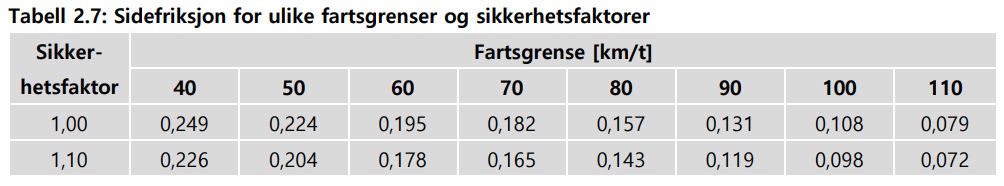
\includegraphics[scale=0.32]{fig/tab2_7}
\end{figure}
\newpage
\op{opgstorstar} 
\tagop{
	\# modellering \# areal \# derivasjon
}
Gitt et rektangel med omkrets $ O $, og la $ x $ være den éne sidelengden.
\abc{
	\item  Finn uttrykket til funksjonen $ A(x) $, som viser aralet til rektangelet.
	\item Hvilken form har rektangelet når arealet er størst?
}

\op{opgmagnskal}
\tagop{
\#logaritmer \#overslag
}
\outl{Momentmagnitudeskalaen} er en skala som brukes til å representere styrken på jordskjelv. Hvis $ S $ er det målte \outl{seismiske momentet} til jordskjelvet, er massemagnituden $ M_w $ gitt som\footnote{Kilde: \net{https://en.wikipedia.org/wiki/Moment_magnitude_scale}{Wikipedia}.}
\[ M_w=\frac{2}{3} \log S-10.7 \]
Energien som jordskjelvet utløser er tilnærmet proporsjonal med $ S $.\os

Gitt to jordskjelv, jordskjelv $ A $ og jordskjelv $ B $, med henholdsvis seismisk moment $ S_A $ og $ S_B $. Si videre at proporsjonalitetskonstanten for energi utløst av det seismiske momentet er likt for begge jordskjelvene. Hvis jordskjelv $ A $ er målt til 1 mer enn jordskjelv $ B $ på momentmagnitudeskalaen, hva er da forholdet mellom energi utløst av jordskjelv $ A $ og energi utløst av jordskjelv $ B $? 
\newpage
\op{opgkast}
Du skal prøve å kaste en ball så langt som mulig langs et flatt strekke. Posisjonen ballen har idét den forlater handen din setter du til $ (0, 0) $. Ved å anta at tyngdekraften deretter er den eneste kraften som virker på ballen, er posisjonen til ballen godt tilnærmet ved uttrykket
\[ \vec{p}_g(t)=\vec{v}t-[0, 5t^2] \]
hvor $ \vec{v}=[v_0 \cos \theta, v_0 \sin \theta] $ er hastighetsvektoren til ballen idét den forlot handen, og $ t $ er antall tidsenheter etter at ballen har forlatt handen. Idét ballen forlater handen din har den farten $ v_0 $, $ \vec{v} $ danner vinkelen $ \theta $ med horisontallinjen.\vsk 

Ut ifra $ \vec{p}_g $, hvilken verdi må $ \theta $ ha for at kastet skal bli lengst mulig?

\op{opgveiformel}
\tagop{
\# integrasjon \# derivasjon
}
La funksjonen $ s(t) $ beskrive hvor langt et objekt har bevegd seg etter tiden $ t $. Hvi objektet har konstant akselerasjon $ a $, har vi at
\[ s''(t)=a \] 
\abc{
\item Integrer $ s''(t) $ to ganger slik at du ender opp med et uttrykk for $ s(t) $.
\item Bestem uttrykkene for $ s(t) $ og $ s'(t) $ når du vet at $ s(t)=0 $ og $ s'(t)=v_0 $.
\item Hvilken fysisk størrelse representerer $ s'(t) $?
\item Undersøk begrepet ''bevegelsesligninger''\footnote{''Eqautions of motion på engelsk.} (også kalt ''veiformler'') i en fysikkbok eller på internett. Sammenlign uttrykkene du finner med uttrykket du fant for $ s(t) $. 
}
\newpage
\op{opgbane}
\tagop{
\#vektorer i planet \#derivasjon
}
Posisjonen $ \vec{s} $ til et objekt som beveger seg i en sirkelbane kan uttrykkes som 
\[ \vec{s} = r[\cos\left(2\pi f t\right), \sin\left(2\pi f t\right)] \]
hvor $ r $ er radien til sirkelbanen, $ t $ er tiden og $ f $ er frekvensen. 
\abc{
\item $ f $ beskriver antall runder objektet fullfører per tidsenhet\footnote{Hvis tidsenheten er 'sekund', har $ f $ benevningen '1/sekund'.}. Forklar hvorfor $ 2\pi f $ kalles \outl{vinkelfarten} til objektet.
\item Finn $ \vec{s}\,'(t) $. 
\item Hva er vinkelen mellom $ \vec{s}(t) $ og $ \vec{s}\,'(t) $?
\item Bestem lengden til $ \vec{s}\,'(t) $
\item Finn $ \vec{s}\,''(t) $.
\item Bestem lengden til $ \vec{s}\,''(t) $
\item  Hva er vinkelen mellom $ \vec{s}(t) $ og $ \vec{s}\,''(t) $? Peker $ \vec{s}\,''(t) $ innover i sirkelbanen eller ut fra sirkelbanen?
\item Bruk en fysikkbok eller internett til å undersøke begrepet \outl{sentripetalakselerasjon}. Sammenlign funnene dine i denne oppgaven med informasjonen du finner.
}

\newpage
\op{opgfloogfjere}
\tagop{\# trigonometri}
En tilnærming for høy- og lavvann i Molde er gitt ved \\funksjonen 
\[ f(x)=128+80\cos\left(\frac{3\pi}{37}x\right) \]
hvor $ f $ angir cm over sjøkartnull\footnote{Sjøkartnull er som regel satt til den laveste vannstanden som kan oppnås ut ifra astronomiske betingelser (flo og fjære er i stor grad betinget av hvordan jorda, sola og månen står i forhold til hverandre).} $ t $ timer etter et gitt referanse-tidspunkt. Referansetidspunktet er valgt slik at det ved $ {t=0} $ var høyvann (flo). \os
\abc{
\item Hva er vannstanden i Molde når det er lavvann (fjøre)?\os
\item Hvor lang tid er det mellom flo og fjøre? 
}
\mers{Denne oppgaven kan med fordel løses uten digitale hjelpemidler.}

\newpage
\section{Teoretiske utvidelser}
\op{opgintpi}
Gitt funksjonen
\[ f(x)=\sqrt{1-x^2} \]
\abc{
\item Finn $ g(x)=f'(x) $.
\item I \tmto\, er formelen for lengden $ l $ til en graf gitt. Forklar hvilket tall $ l $ representerer når $ f $ og $ g $ er som gitt i denne oppgaven, $ a=-1 $ og $ b=1 $.
\item Bruk en numerisk metode til for å finne en tilnærming for $ l $. Drøft på forhånd hvilke hensyn som må tas for å unngå at skriptet feiler ved kjøring.
}

\section{Praktiske oppgaver}
\section{Eksamensoppgaver}
\end{document}

